\documentclass{article}
\usepackage{graphicx}
\usepackage[utf8]{inputenc}

\graphicspath{ {./images/} }

\title{Dissertation}
\author{Quentin Sonnefraud}
\date{July 2020}

\begin{document}

\maketitle


\section{Introduction}

\section{Overview of some changepoint detection algorithm and application of classifcation of warmup analysis}

\section{ How to detect the change between benchmarks ? Overwiew of method to quantify difference between curve}

DUring this project I have review and try some techniques to quantify the difference between benchmarks and report if changement of behavior as occure

\subsection{Area method}

First i have used area method to quantify the difference between curve, this an algorithm for calculating the Area between two curves in 2D space
Strictly speaking, the expression area under the curve refers to the area A of the domain delimited by a curve (represented in an x-y diagram) and three straight lines (the x-axis and two vertical lines with abscissa a and b). If the curve has the equation $y=f(x)y=f(x)$, the area is $\dA=\int _{a}^{b}f(x)\,\mathrm {d} x$. This area is a true area (e.g. milliseconds for benchmarks) only if the function f has only positive (or zero) values over the interval [a,b] and if both the abscissa and the ordinate are lengths (with the same choice of unit, e.g. milliseconds for benchmarks).
For the purpose of detecting if the behaviour has change between two benchmarks its not interesting because it quantify the area a a whole and area can be equal but not their behaviour

\subsection{Hausdorff Distance }
The Hausdorff distance is used to account for the maximum deviation between two polylines (L1, L2) (Taha and Hanbury 2015). By definition, two polylines L1 and L2 are at a Hausdorff distance (dH) from each other of less than d units, if each point of L1 is within d units of at least one point of L2, and if, reciprocally, each point of L2 is less than d units away from each other by at least one
point of L1.

The Hausdorff distance is defined as the greater of the two following components :
\begin{itemize}
    \item d1 which is the largest value of the non-symmetrical distance from L1 to L2,
    \item d2 which is the largest value of the non-symmetrical distance from L2 to L1.
\end{itemize}


This distance has the advantage of providing two measurements. Right-of-way lines can thus be compared using the component starting from the most short line. On the other hand, the Hausdorff distance, with the disadvantage of calculating the
distance on the nearest pairs of points and not on homologous points. Homologous points are points that visually correspond to each other. For example, the point in L2 used to calculate d1 is not the Intuitively corresponding to the point of L1, it is simply the closest point. The distance from Hausdorff considers polylines as simple sets of dots unordered. This problem is particularly important for very sinuous or with loops. Small distances can then be sent back to dissimilar lines. Similarly, pairs of dots cannot be considered to be matches. Nevertheless, this particularity has the advantage of
reduce calculation time: the algorithmic complexity of this algorithm is linear (Taha and Hanbury 2015). 


This methods seems to be working better because there is no need for the dataset to know if the first clue of the first sequence must match the first clue of the other sequence and that
the last clue of the first sequence must match the last clue of the other sequence (but it must not be its only match).

\subsection{Fréchet distance}
I have presented a discrete variant of the Fréchet distance between curves in a metric
space, and they described a simple and efficient algorithm for computing this measure.
Besides its own interest, discrete Fréchet distance may be used for approximately computing the Fréchet distance between two arbitrary curves, as an alternative to using the exact Fréchet distance between a polygonal approximation of the curves or an approximation of this value

\subsection{DTW}

The DTW has been widely used in speech recognition to align speech segments of different speakers. The strategy applied by the algorithm is This is very similar to the technique used for text comparison. The DTW finds the best match between a reference (the score) and a signal (the interpretation) by calculating a difference between vectors of the characteristics for each of these signals. The comparison algorithms of chaines are based on the exact correspondence between the reference and the signal and do not take into account, among other things, the imprecision of the pitch estimation due to chords or errors of the height detection algorithm. In addition, the DTW can be used to align continuous multi-dimensional characteristics, for example results from a signal analysis, which allows the partition alignment to be based on parameters such as the number of partitions, the size of the partition, the number of partitions, the number of partitions to be aligned, the number of partitions to be aligned, the number of partitions to be aligned, the number of partitions to be aligned and the number of partitions to be aligned.
The system does not require prior segmentation of the benchmark measurements and does not require prior segmentation of the
signal.
In short, the DTW algorithm consists of three steps:

\begin{itemize}
    \item Calculation of local distances
    \item Dynamic programming to obtain the global optimum \begin{itemize}
        \item a) Calculation of increased distances. Only the minimum predecessors are kept. of each point => local optimum
        \item b) Backtrack to find the minimum distance => global optimum
    \end{itemize}
    \item Result: A shift path that consists of the correspondence of the two equations.

    
\end{itemize}

\subsection{Interpretation of results after running the algorithms}

\begin{figure}[h]
    \centering
    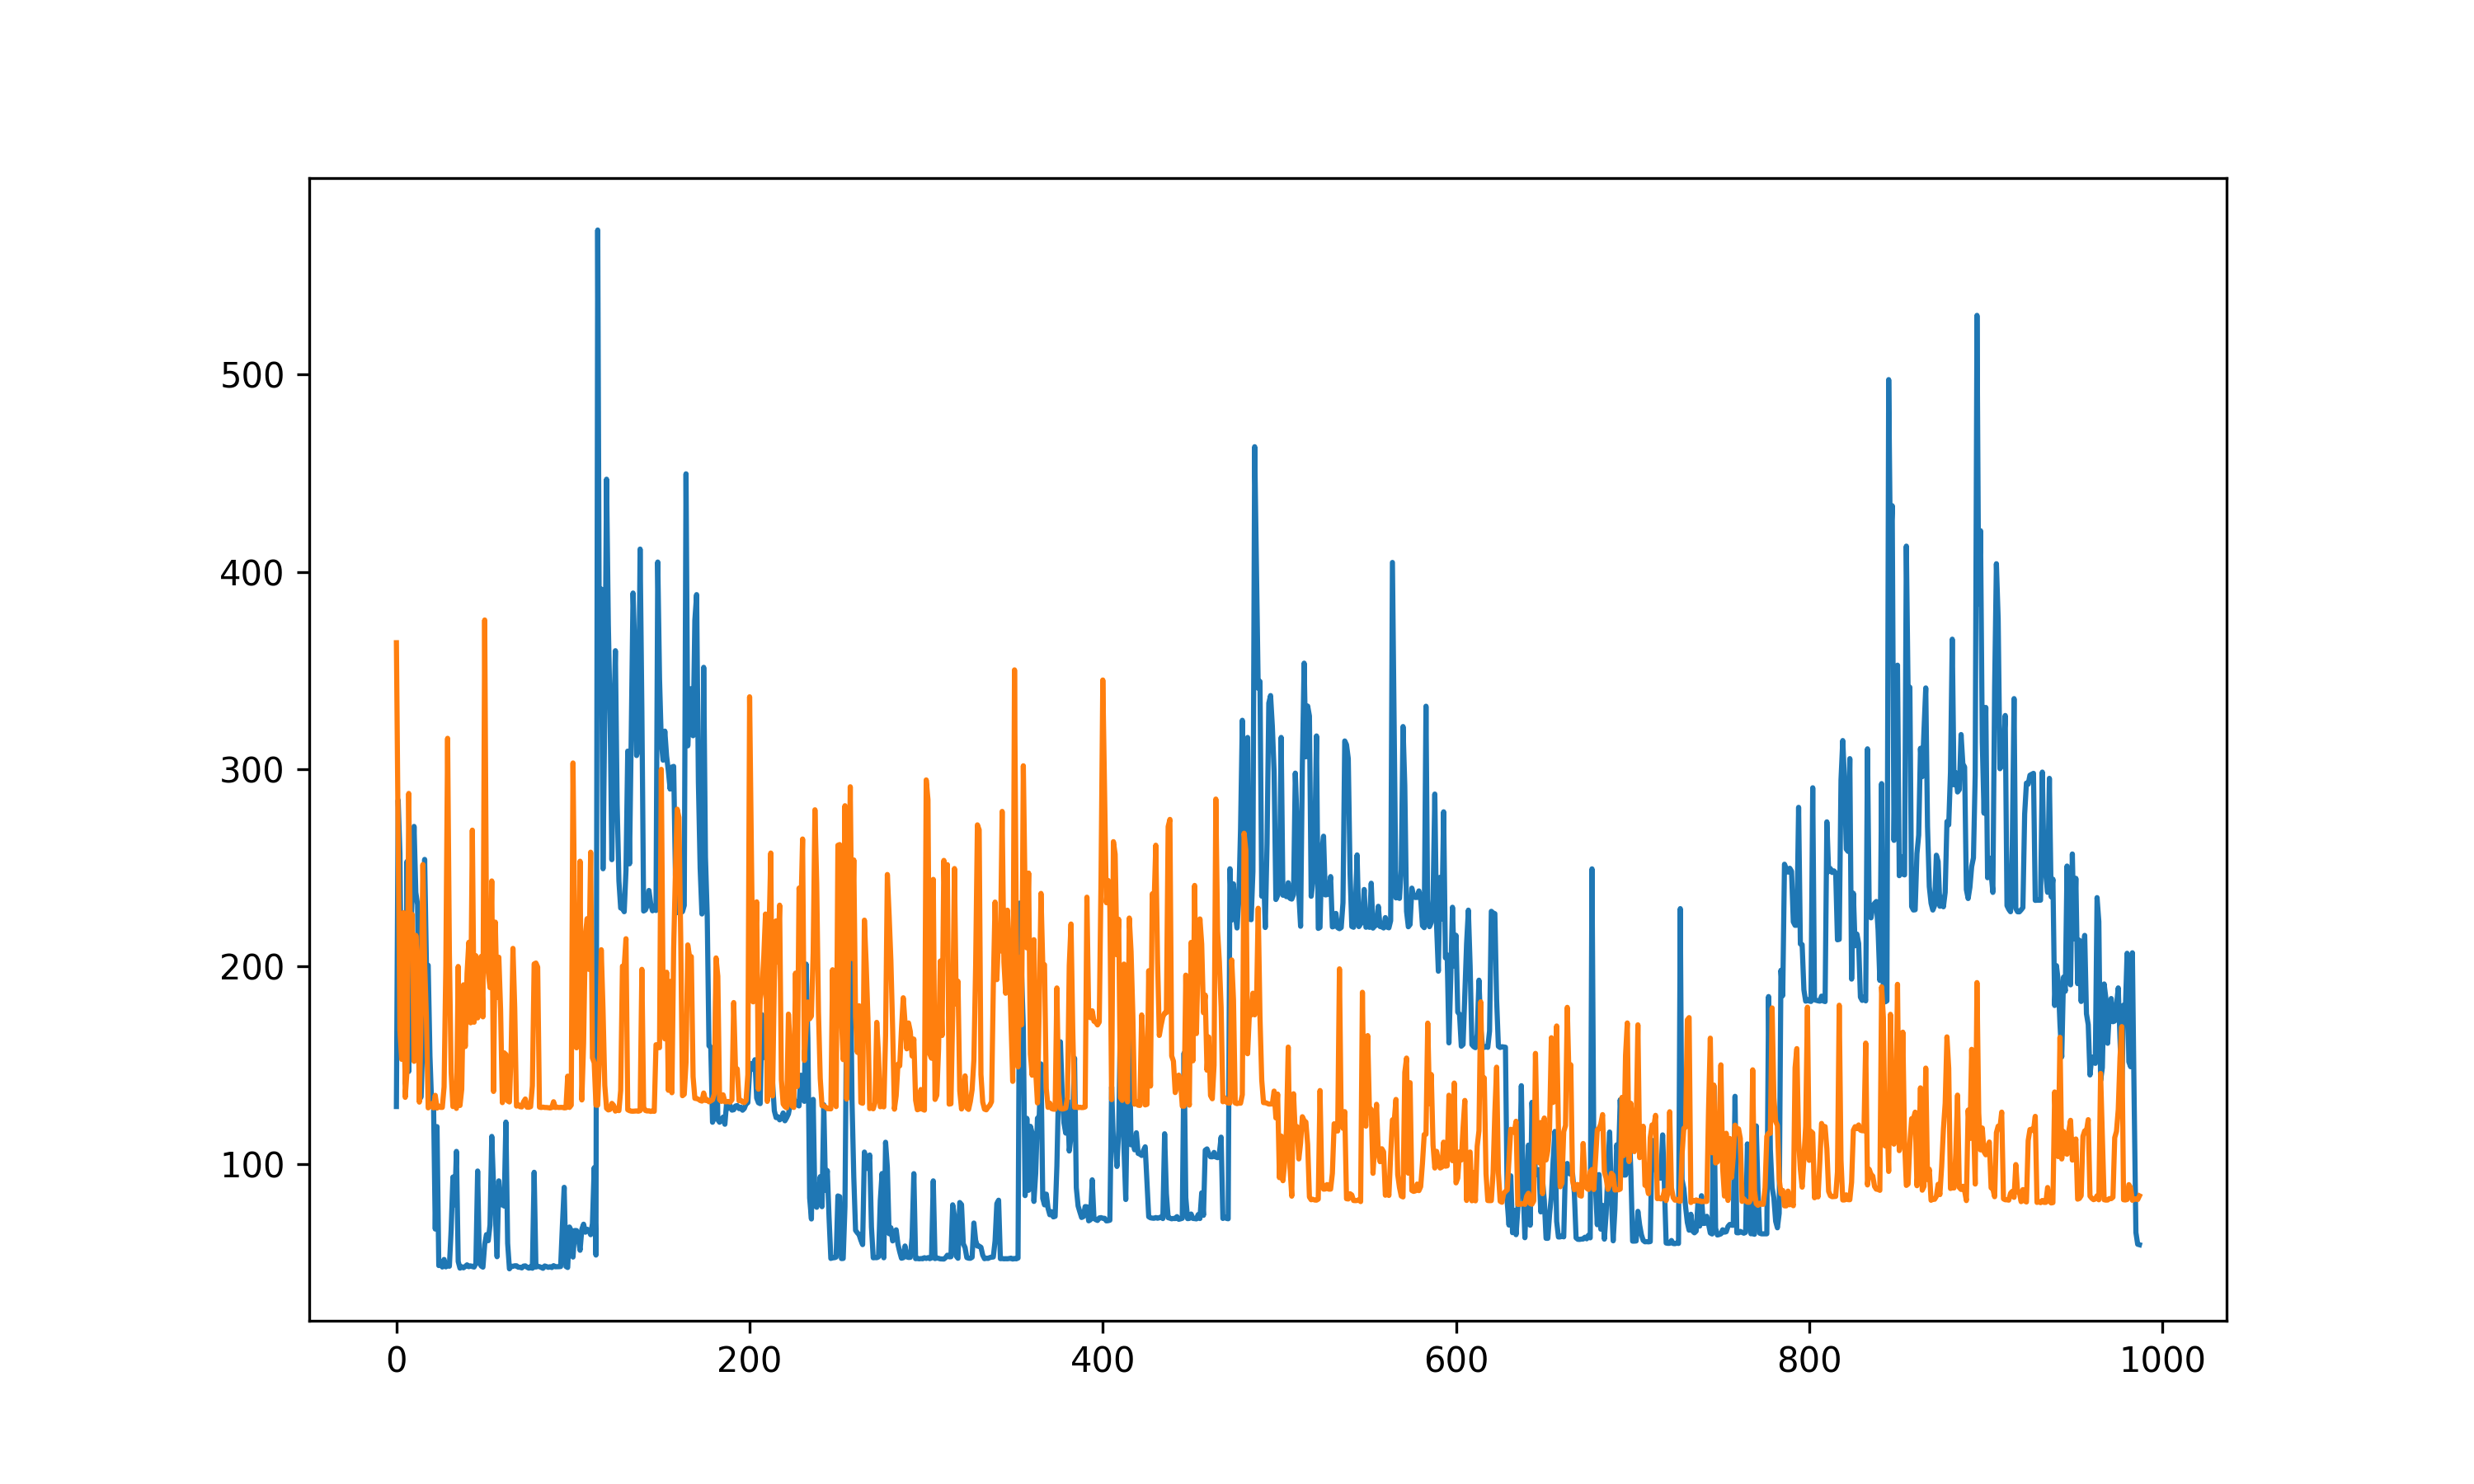
\includegraphics[width=1\textwidth]{plot_0.png}
    \caption{Benchmark 1 and 2 From sleeping Barber}
    \label{fig:mesh1}
\end{figure}


\begin{figure}[h]
    \centering
    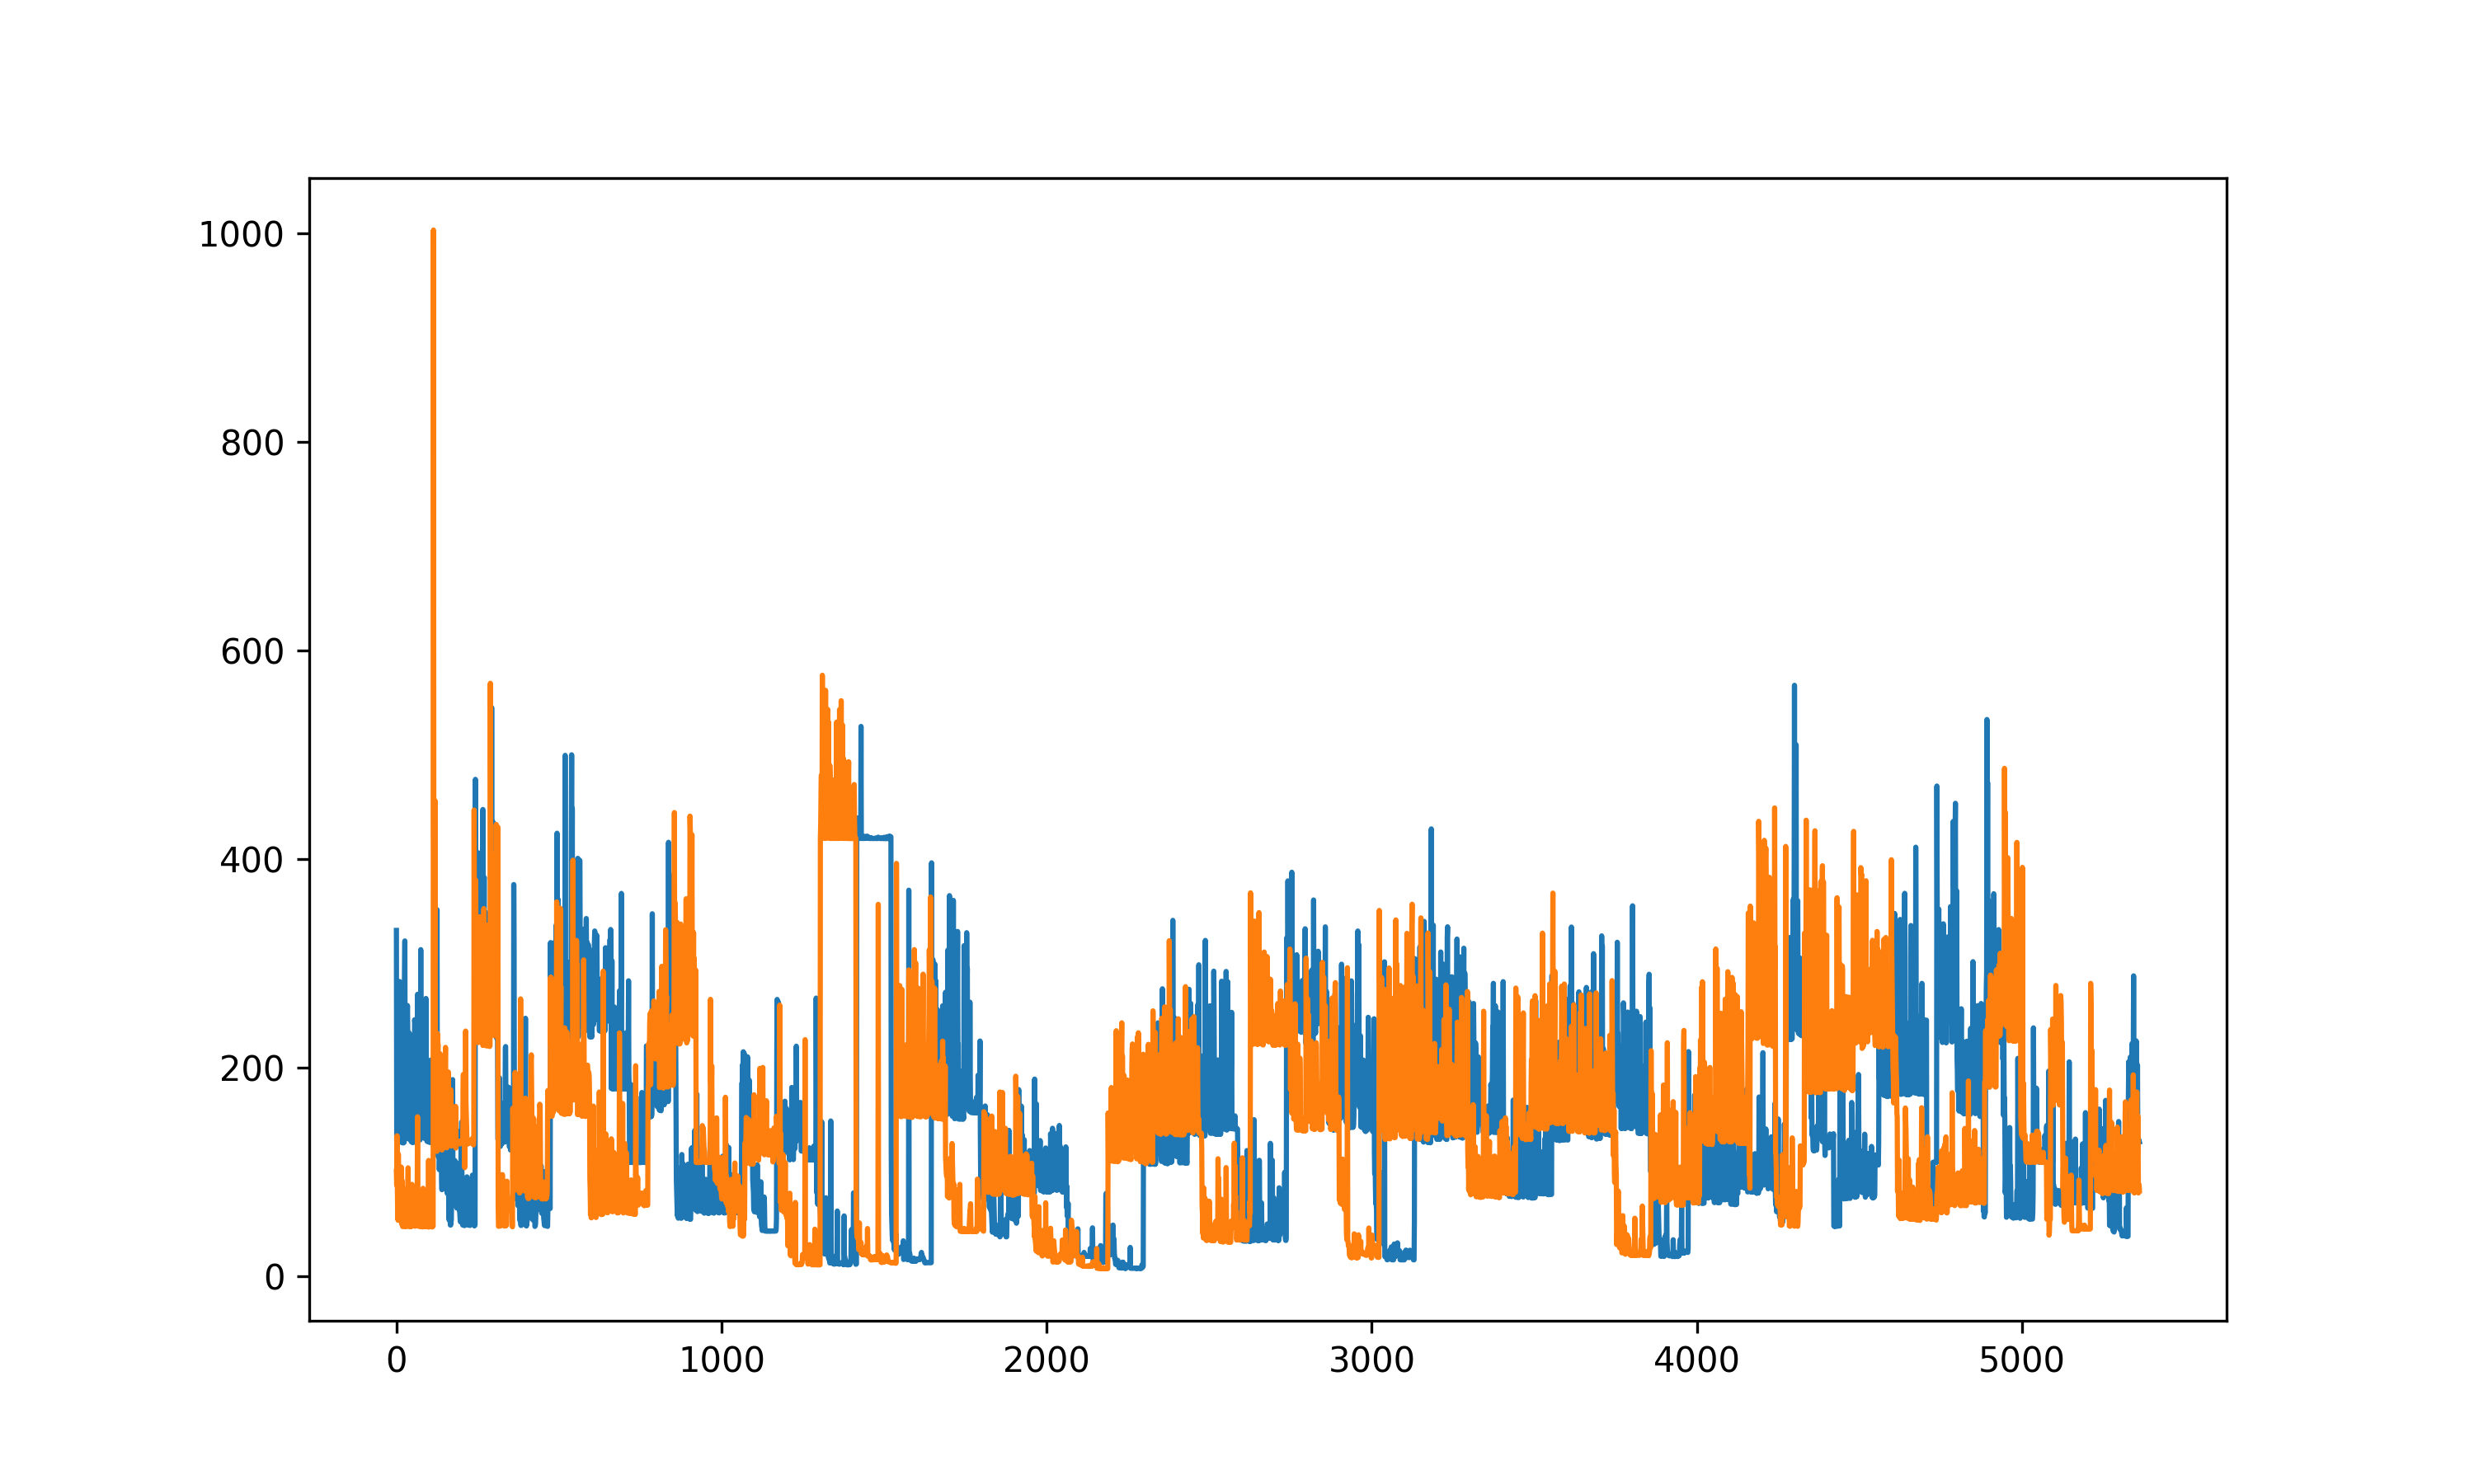
\includegraphics[width=1\textwidth]{plot_1.png}
    \caption{Benchmark 2 and 3 From sleeping Barber}
    \label{fig:mesh1}
\end{figure}

\begin{table}[h!]
\begin{tabular}{|l|c|c|c|c|c|c|}
   \hline
   benchmarks & pcm & frechet distance & area & curve length & DTW & directed hausdorf \\
   \hline
   1 \&  2 & 132 & 313 & 81918 & 14 & 68757 & 197\\
   \hline
   2 \& 3 & 573 & 295 & 32960 & 48 & 191649 & 7 \\
   \hline
\end{tabular} \\ 
\caption{Comparaison between two inequal benchmarks and two equal benmarks}
\end{table}


As expected the only algorithm that seems to work is the directed hausdorf algorithm because it is not influence by the size of the dataset, indeed as the curve lenght increase the difference of the score increase. 
I have put a treshold of 20 with the directed hausdorf. When the direcred hausdorf value is more than 20 is interesting to look at the benchmark because it means that their is significant difference between the two benchmarks.

\subsection{Conclusion of classification of changement of behaviour between benchmarks}

The validation of an unsupervised classification, as well as the choice of the number of group always remain open questions. On real data, recognized criteria such as the distance difference or the silhouette index are optimal with only two groups, limiting the contribution of such an analysis.








\end{document}
